\documentclass[conference]{IEEEtran}
% Some/most Computer Society conferences require the compsoc mode option,
% but others may want the standard conference format.


% *** CITATION PACKAGES ***
% 
\ifCLASSOPTIONcompsoc
% IEEE Computer Society needs nocompress option
% requires cite.sty v4.0 or later (November 2003)
\usepackage[nocompress]{cite}
\else
% normal IEEE
\usepackage{cite}
\fi
% cite.sty was written by Donald Arseneau
% V1.6 and later of IEEEtran pre-defines the format of the cite.sty package
% \cite{} output to follow that of the IEEE. Loading the cite package will
% result in citation numbers being automatically sorted and properly
% "compressed/ranged". e.g., [1], [9], [2], [7], [5], [6] without using
% cite.sty will become [1], [2], [5]--[7], [9] using cite.sty. cite.sty's
% \cite will automatically add leading space, if needed. Use cite.sty's
% noadjust option (cite.sty V3.8 and later) if you want to turn this off
% such as if a citation ever needs to be enclosed in parenthesis.
% cite.sty is already installed on most LaTeX systems. Be sure and use
% version 5.0 (2009-03-20) and later if using hyperref.sty.
% The latest version can be obtained at:
% http://www.ctan.org/pkg/cite
% The documentation is contained in the cite.sty file itself.
% 
% Note that some packages require special options to format as the Computer
% Society requires. In particular, Computer Society  papers do not use
% compressed citation ranges as is done in typical IEEE papers
% (e.g., [1]-[4]). Instead, they list every citation separately in order
% (e.g., [1], [2], [3], [4]). To get the latter we need to load the cite
% package with the nocompress option which is supported by cite.sty v4.0
% and later.




\usepackage[pdftex]{graphicx}
\graphicspath{{./png/}{./eps/}}
\DeclareGraphicsExtensions{.pdf,.jpeg,.png,.eps}

% *** GRAPHICS RELATED PACKAGES ***
% 
\ifCLASSINFOpdf
% \usepackage[pdftex]{graphicx}
% declare the path(s) where your graphic files are
% \graphicspath{{../pdf/}{../jpeg/}}
% and their extensions so you won't have to specify these with
% every instance of \includegraphics
%\DeclareGraphicsExtensions{.pdf,.jpeg,.png}
\else
% or other class option (dvipsone, dvipdf, if not using dvips). graphicx
% will default to the driver specified in the system graphics.cfg if no
% driver is specified.
% \usepackage[dvips]{graphicx}
% declare the path(s) where your graphic files are
% \graphicspath{{../eps/}}
% and their extensions so you won't have to specify these with
% every instance of \includegraphics
% \DeclareGraphicsExtensions{.eps}
\fi
% graphicx was written by David Carlisle and Sebastian Rahtz. It is
% required if you want graphics, photos, etc. graphicx.sty is already
% installed on most LaTeX systems. The latest version and documentation
% can be obtained at: 
% http://www.ctan.org/pkg/graphicx
% Another good source of documentation is "Using Imported Graphics in
% LaTeX2e" by Keith Reckdahl which can be found at:
% http://www.ctan.org/pkg/epslatex
% 
% latex, and pdflatex in dvi mode, support graphics in encapsulated
% postscript (.eps) format. pdflatex in pdf mode supports graphics
% in .pdf, .jpeg, .png and .mps (metapost) formats. Users should ensure
% that all non-photo figures use a vector format (.eps, .pdf, .mps) and
% not a bitmapped formats (.jpeg, .png). The IEEE frowns on bitmapped formats
% which can result in "jaggedy"/blurry rendering of lines and letters as
% well as large increases in file sizes.
% 
% You can find documentation about the pdfTeX application at:
% http://www.tug.org/applications/pdftex


% *** MATH PACKAGES ***
\usepackage{amsmath}
\interdisplaylinepenalty=2500

% *** SPECIALIZED LIST PACKAGES ***
% 
% \usepackage{algorithmic}
% algorithmic.sty was written by Peter Williams and Rogerio Brito.
% This package provides an algorithmic environment fo describing algorithms.
% You can use the algorithmic environment in-text or within a figure
% environment to provide for a floating algorithm. Do NOT use the algorithm
% floating environment provided by algorithm.sty (by the same authors) or
% algorithm2e.sty (by Christophe Fiorio) as the IEEE does not use dedicated
% algorithm float types and packages that provide these will not provide
% correct IEEE style captions. The latest version and documentation of
% algorithmic.sty can be obtained at:
% http://www.ctan.org/pkg/algorithms
% Also of interest may be the (relatively newer and more customizable)
% algorithmicx.sty package by Szasz Janos:
% http://www.ctan.org/pkg/algorithmicx




% *** ALIGNMENT PACKAGES ***
% 
% \usepackage{array}
% Frank Mittelbach's and David Carlisle's array.sty patches and improves
% the standard LaTeX2e array and tabular environments to provide better
% appearance and additional user controls. As the default LaTeX2e table
% generation code is lacking to the point of almost being broken with
% respect to the quality of the end results, all users are strongly
% advised to use an enhanced (at the very least that provided by array.sty)
% set of table tools. array.sty is already installed on most systems. The
% latest version and documentation can be obtained at:
% http://www.ctan.org/pkg/array

\hyphenation{op-tical net-works semi-conduc-tor}

\begin{document}
\title{A Proposal for an Intuitionistic Fuzzy Inference System}


\author{\IEEEauthorblockN{Amaury Hernandez-Aguila, Mario
    Garcia-Valdez, Oscar Castillo}
  \IEEEauthorblockA{Tijuana Institute of Technology\\
    Division of Graduate Studies and Graduates\\
    Tijuana, Mexico\\
    Email: \{amherag,mario,ocastillo\}@tectijuana.edu.mx}}

\maketitle

\begin{abstract}

\end{abstract}

\IEEEpeerreviewmaketitle



\section{Introduction}

What is a fuzzy set? \cite{zadeh1965fuzzy}

What is fuzzy logic? \cite{klir1995fuzzy}

Types of fuzzy sets. Mendel book \cite{mendel2001uncertain}

What is a fuzzy inference system?

There can be different types. Type-2 \cite{mendel2002type}, interval
t2 \cite{liang2000interval} and \cite{mendel2006interval}

Type-2 is time-consuming. Shadowed sets \cite{pedrycz1998shadowed}

What is a intuitionistic fuzzy set? \cite{atanassov1986intuitionistic}
\cite{atanassov2003intuitionistic} \cite {despi2013generalised}

\section{Related Work}

Application of intuitionistic fuzzy sets, bacillus colonies
recognition \cite{davarzani2013novel}

Alpha cut \cite{sharma2011cut} \cite{sharma2011cutgroups}

intuitionistic inference engine \cite{cornelis2001compositional}

implementation of a ifis, castillo \cite{castillo2007intuitionistic}

more inference \cite{bustince1995method}

centroid of a type-2 fuzzy-set \cite{karnik2001centroid}

and even more inference \cite{marinov2005method}

Intuitionistic control washing machines \cite{akram2014intuitionistic}

\section{Preliminaries}

Define in more detail intuitionistic fuzzy sets. 

Formulas and basic explanation (below) \cite{atanassov2013intuitionistic}

% intuitionistic fuzzy set
\begin{equation}
  A^{*} = \{\langle x, \mu _{A} (x), \nu _{A} (x) \rangle | x \in E\}
\end{equation}

% intuitionistic interval
\begin{equation}
  \label{intuitionistic-interval}
  0 \leq \mu_{A}(x) + \nu_{A}(x) \leq 1
\end{equation}

% every ordinary fuzzy set has the form
\begin{equation}
  \label{ifs-form}
  \{ \langle x, \mu_{A}(x), 1 - \mu_{A}(x) \rangle | x \in E \}
\end{equation}

% if
\begin{equation}
  \label{fs-as-ifs-if}
  \pi_{A}(x) = 1 - \mu_{A}(x) - \nu_{A}(x)
\end{equation}

\section{Proposed Method}

The method, for now, consists on the procedures and elements
necessary to construct a basic Intuitionistic Fuzzy Inference System
(IFIS). This design was completed in order to make comparisons against
classic Fuzzy Inference Systems (FISs), such as Type-1 FIS, Interval
Type-2 and General Type-2 FIS, and prove that
the design was viable and able to contribute to better results than
the classic FISs.

In many works, intuitionistic fuzzy sets (IFSs) are constructed by
hand, by interviewing experts who assign memberships and
non-memberships to each of the values of a set (such as in
\cite{davarzani2013novel}). This work proposes a convenient way of
creating an IFS, imitating many systems that use Gaussian
membership functions (MFs) to facilitate an expert the representation of a
fuzzy interpretation. An example of an IFS is depicted in
Fig. \ref{fs-as-ifs}. This IFS represents a classic fuzzy set, as it
satisfies (\ref{ifs-form}) and (\ref{fs-as-ifs-if}), by representing
the MF as the red line, and the non-membership
function (NMF) as the blue line. In order to contruct the NMF, one has
to rotate a normal Gaussian MF by 180˚, and this can be seen as the
complement of the fuzzy set corresponding to a Gaussian MF.

\begin{figure}[!t]
  \centering
  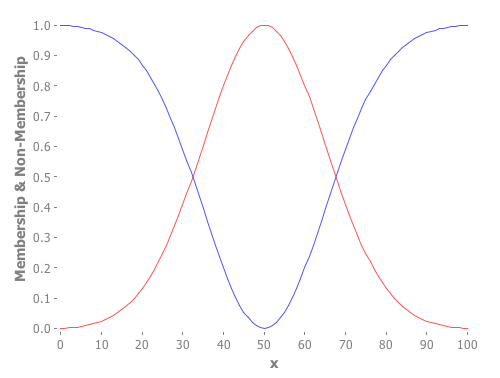
\includegraphics[width=2.5in]{fs-as-ifs}
  \caption{Classic Fuzzy Set Represented as an Intuitionistic Fuzzy Set}
  \label{fs-as-ifs}
\end{figure}

Two convenient ways of modifying the NMF and
satisfy (\ref{intuitionistic-interval}) are as follows: 1) one can set
the mean and the standard deviation of the Gaussian functions to be
the same, and only vary the $height$ of the NMF,
as is depicted in Fig. \ref{ifs}; and 2) one can set different means and
standard deviations of the Gaussian membership and non-membership
functions, but the $height$ of the MF must be equal
to $h_{mf} = 1 - h_{nmf}$, as this ensures that
(\ref{intuitionistic-interval}) is satisfied. An example of the latter
case is shown in Fig. \ref{ifs-diff-mu-sd}. To clarify, the $height$
of the MF ($h_{mf}$) of an IFS is equal to $max(\mu(x))$, and the
$height$ of the NMF ($h_{nmf}$) of an IFS is equal to $max(\nu(x))$.

\begin{figure}[!t]
  \centering
  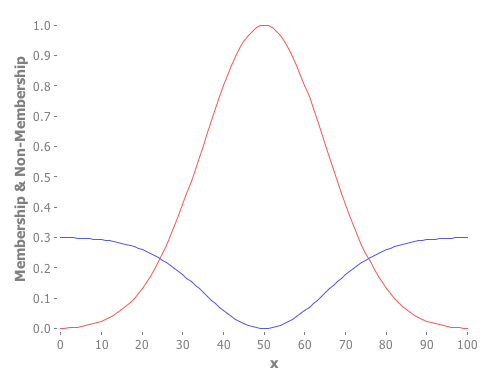
\includegraphics[width=2.5in]{ifs}
  \caption{An Example of an Intuitionistic Fuzzy Set - Same Mean and SD}
  \label{ifs}
\end{figure}

\begin{figure}[!t]
  \centering
  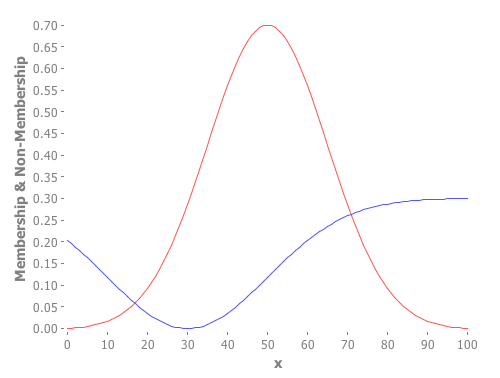
\includegraphics[width=2.5in]{ifs-diff-mu-sd}
  \caption{An Example of an Intuitionistic Fuzzy Set - Different Mean
    and SD}
  \label{ifs-diff-mu-sd}
\end{figure}

The first step in an inference process in a classic FIS (a flow chart
for the process in an IFIS is given in Fig. \ref{flow-chart}) is to
determine what membership corresponds to a given input, given a set of
MFs. This is straightforward in a classic FIS, as the
membership to each input is already established in the membership
fuzzy set. For an IFIS, this work proposes a method to determine a
membership given a MF and a NMF,
which is described in (\ref{imembership}), and receives the name of
$i\mu$ (intuitionistic membership).

\begin{figure}[!t]
  \centering
  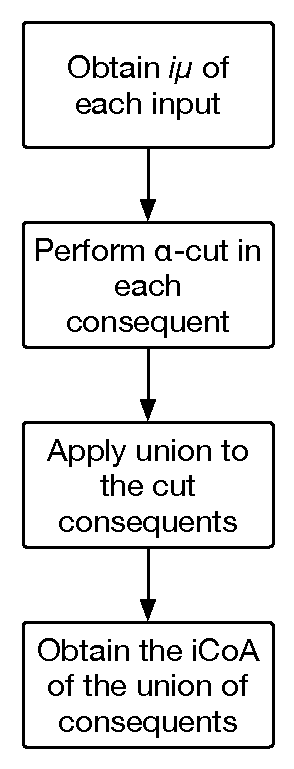
\includegraphics[height=2.5in]{proposed-method-flow-chart}
  \caption{Proposed Method Flow Chart}
  \label{flow-chart}
\end{figure}

% i-membership
\begin{equation}
  \label{imembership}
  i\mu_{A}(x) = (\nu_{A}(x) + \mu_{A}(x))\mu_{A}(x)
\end{equation}

A comparison of a MF (red line) against an intuitionistic
membership function (blueline) is shown in Fig.
\ref{if-membership}. The parameters for both the MF and NMF are $\mu =
50$ and $SD = 15$, but the $height$ for the NMF is set at $0.5$. This
results in an intuitionistic MF that appears to have the same mean,
but a smaller standard deviation. A more elaborated example is shown
in Fig. \ref{if-membership-drastic}, where the parameters of the MF
are $\mu = 50$, $SD = 15$ and $h = 0.8$, and the parameters of the NMF
are $\mu = 30$, $SD = 20$ and $h = 0.2$. As can be noted, the
indeterminacy ($\pi$) is high in this example, which results in a
smaller $SD$ for the intuitionistic MF. Moreover, the difference in
means and standard deviations generates a change of the mean for the
intuitionistic MF.

\begin{figure}[!t]
  \centering
  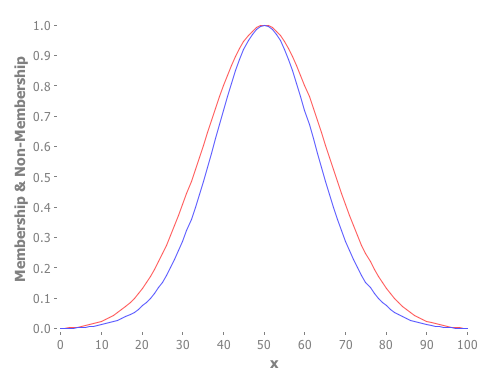
\includegraphics[width=2.5in]{if-membership}
  \caption{Comparison of $\mu(x)$ Against $i\mu(x)$}
  \label{if-membership}
\end{figure}

\begin{figure}[!t]
  \centering
  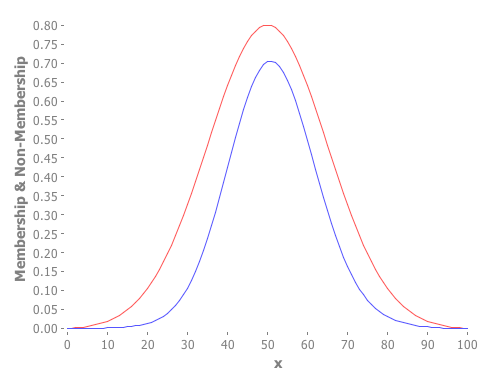
\includegraphics[width=2.5in]{if-membership-drastic}
  \caption{Comparison of $\mu(x)$ Against $i\mu(x)$ With More Indeterminism}
  \label{if-membership-drastic}
\end{figure}

The next step in the inference process is to perform an $\alpha$-cut
on the associated consequents to the antecedents that are activated by
the inputs. In a classic FIS, this process is straightforward, as the
memeberships in a fuzzy set representing a consequent are ``cut'' by
following (\ref{alpha-cut}) for every element in a fuzzy set
representing a consequent. In an intuitionistic MF, one can follow
the same procedure in order to obtain the $\alpha$-cut in the MF part,
but to obtain the $\alpha$-cut in the NMF, (\ref{nmf-alpha-cut}) must
be followed. In (\ref{nmf-alpha-cut}), the counterintuitive part is
that one has to find the corresponding $\nu$ for a given
$\mu_{\alpha}$. An example of an $\alpha$-cut, with $\mu_{\alpha} =
0.6$, is depicted in Fig. \ref{alpha-cut-example}.

\begin{equation}
  \label{alpha-cut}
  \alpha(\mu (x),\mu_{\alpha}) =
  \begin{cases}
    \mu (x), & \text{if}\ \mu (x) \leq \mu_{alpha}  \\
    \mu_{\alpha}, & \text{otherwise}
  \end{cases}
\end{equation}

\begin{equation}
  \label{nmf-alpha-cut}
  \alpha_{NMF}(\nu (x),\mu_{\alpha}) =
  \begin{cases}
    \nu (x), & \text{if}\ \nu (x) \geq \nu (\mu_{alpha})  \\
    \nu (\mu_{alpha}), & \text{otherwise}
  \end{cases}
\end{equation}

\begin{figure}[!t]
  \centering
  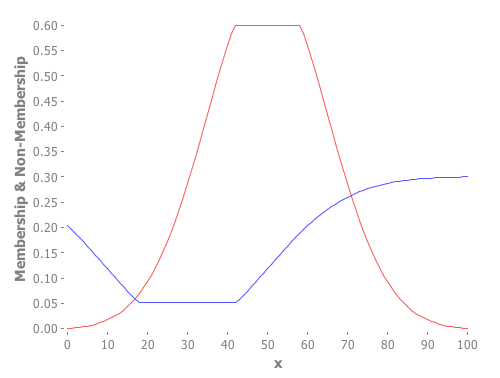
\includegraphics[width=2.5in]{alpha-cut}
  \caption{$\alpha$-cut of an Intuitionistic Fuzzy Set}
  \label{alpha-cut-example}
\end{figure}

After performing every necessary $\alpha$-cut, one has to apply the
union operator over every resulting fuzzy set, in order to aggregate
the weights of all the consequents. The union operator is defined by
K. Atanassov \cite{atanassov2013intuitionistic}, for every two IFSs A
and B, as in (\ref{union-operator}). An example of an union of three
IFSs is shown in Fig. (\ref{ifs-union}).

\begin{equation}
  \label{union-operator}
  \begin{aligned}
    A \cup B  = &\{ \langle x, max(\mu_{A} (x), \mu_{B} (x)),\\
    &\quad min(\nu_{A} (x), \nu_{B} (x)) \rangle | x \in E \}
\end{aligned}
\end{equation}

\begin{figure}[!t]
  \centering
  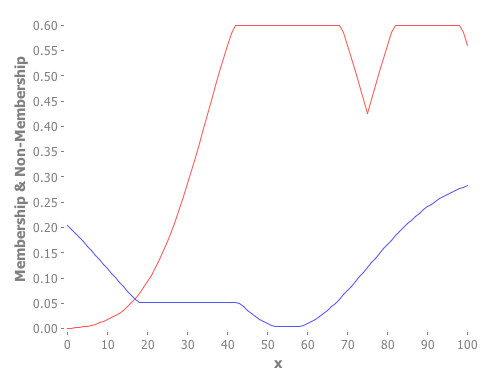
\includegraphics[width=2.5in]{ifs-union}
  \caption{Union of Three $\alpha$-cut Intuitionistic Fuzzy Sets}
  \label{ifs-union}
\end{figure}

Finally, one has to defuzzify the aggregation of the $\alpha$-cut
consequents, in order to obtain a crisp number that represents
it. There are a number of methods that can be used to defuzzify a
fuzzy set, but the most frequently found in the literature is the
Center of Area (CoA), or simply centroid. One can obtain the centroid
of a classic fuzzy set A by using (\ref{center-of-area}). For an
IFS, one can use the concept of intuitionistic membership ($i\mu$) and
extend (\ref{center-of-area}) to obtain (\ref{if-coa}). By
substituting $(\mu(x_{i}) + \nu(x_{i}))$ by $i\mu_{A}$, one arrives at
(\ref{if-coa-simplified}), which is a simplification of (\ref{if-coa}).

% CoA
\begin{equation}
  \label{center-of-area}
  A_{CoA} = \dfrac{\sum_{i=1}^{N} \mu(x_{i})
    x_{i}}{\sum_{i=1}^{N} \mu(x_{i})}
\end{equation}

%iCoA
\begin{equation}
  \label{if-coa}
  A_{iCoA} = \dfrac{\sum_{i=1}^{N} (\mu(x_{i}) + \nu(x_{i})) \mu(x_{i})
    x_{i}}{\sum_{i=1}^{N} (\mu(x_{i}) + \nu(x_{i})) \mu(x_{i})}
\end{equation}

%iCoA contracted
\begin{equation}
  \label{if-coa-simplified}
  A_{iCoA} = \dfrac{\sum_{i=1}^{N} i\mu_{A}(x) x_{i}}{\sum_{i=1}^{N}
    i\mu_{A}(x)}
\end{equation}

Fig. \ref{if-coa-vs-coa} shows the plot of the defuzzification of
several IFSs with $CoA$ (red line) and $iCoA$ (blue line), with means set
from 0 to 100 for the MF, and -20 to 80 for the NMF, and standard
deviations of 15 for the MF, and 20 for the NMF.

\begin{figure}[!t]
  \centering
  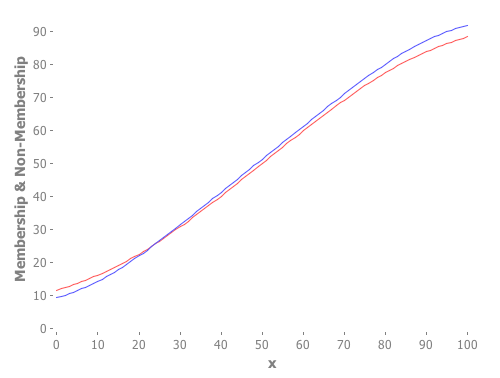
\includegraphics[width=2.5in]{if-coa-vs-coa}
  \caption{Comparison of $CoA_{A_{i}}$ Against $iCoA_{A_{i}}$}
  \label{if-coa-vs-coa}
\end{figure}

\section{Experiments}

The purpose of the experiments in this work is to demonstrate that the
proposed method is viable for performing inference using
intuitionistic fuzzy sets instead of classic fuzzy sets, i.e., that
the concepts of intuitionistic membership ($i\mu$) and intuitionistic
center of area ($iCoA$) enable an extension to traditional fuzzy
inference systems to support indeterminacy and non-membership. To
demonstrate this claim, this work presents a series of experiments
where the proposed method is compared against Type-1 Fuzzy Inference
Systems (T1-FISs) and Interval Type-2 Fuzzy Inference Systems
(T2-FISs) with uncertain mean and uncertain standard deviation.

The initial (and ambitious) hypothesis is that a Type-1 Intuitionistic Fuzzy System (T1-IFIS)
should perform better than a T1-FIS, as it can handle both uncertainty
and indeterminacy, and it is unclear if an IFIS should perform better
than a T2-FIS. The experiments presented in this work
cannot prove this statement profoundly, as the results will only test for a
single situation, which is the prediction of a subset of the
Mackey-Glass time series.

% Comparisons against juzzy \cite{wagner2013juzzy}

% Compare using Mackey-Glass, 100 training, 50 for testing, because it
% took too much time. Genetic algorithm. Present parameters: mean 0-100,
% sd 30-70, mf 1, nmf 0.8-1.0.

% The rule base.

\begin{enumerate}
  \item if $t_{0}$ is $A_{1}$ then $p_{t+1}$ is $C_{1}$
  \item if $t_{-6}$ is $A_{2}$ then $p_{t+1}$ is $C_{2}$
  \item if $t_{-12}$ is $A_{3}$ then $p_{t+1}$ is $C_{3}$
  \item if $t_{-18}$ is $A_{4}$ then $p_{t+1}$ is $C_{4}$
\end{enumerate}

\section{Results}

Results can be found on https://github.com/amherag/wcci-2016-a

\begin{table}[!t]
  \renewcommand{\arraystretch}{1.3}
  \caption{Hypothesis Tests for the Training Stage}
  \label{hypothesis-tests-training}
  \centering
  \begin{tabular}{|c|c|c|c|c|c|}
    \hline
    Method & $\mu_{TR}$ & $SD_{TR}$ & $n$ & t-Value\\
    \hline
    T1 iFIS & 89.50 & 25.36 & 60 & \\
    \hline
    T1 FIS & 108.05 & 23.47 & 60 & -4.1584 \\
    \hline
    IT2 FIS (\(\mu\)) & 112.56 & 29.16 & 100 & -5.2597 \\
    \hline
    IT2 FIS (SD) & 102.31 & 26.08 & 300 & -3.5548 \\
    \hline
  \end{tabular}
\end{table}

\begin{table}[!t]
  \renewcommand{\arraystretch}{1.3}
  \caption{Hypothesis Tests for the Testing Stage}
  \label{hypothesis-tests}
  \centering
  \begin{tabular}{|c|c|c|c|c|c|}
    \hline
    Method & $\mu_{TS}$ & $SD_{TS}$ & $n$ & t-Value\\
    \hline
    T1-iFIS & 160.99 & 65.70 & 60 & \\
    \hline
    T1-FIS & 194.97 & 71.97 & 60 & -2.7010 \\
    \hline
    IT2-FIS (\(\mu\)) & 192.31 & 105.75 & 100 & -2.3104 \\
    \hline
    IT2-FIS (SD) & 178.63 & 99.70 & 300 & -1.7209 \\
    \hline
  \end{tabular}
\end{table}

\section{Conclusion}

This work mainly focuses on proving that the design is viable, but it
also proves that at least in some cases the intuitionistic fis can
out-perform the t1 and t2.

\section{Future Work}

We want to create a toolbox such as \cite{castro2007interval}
We want to experiment with other data sets.
We want to speed up the algorithm.
We want to experiment with generalized type-2.

\bibliographystyle{IEEEtran}
\bibliography{paper}

\end{document}
